\begin{figure*}
    \centering
    \begin{subfigure}{\textwidth}
    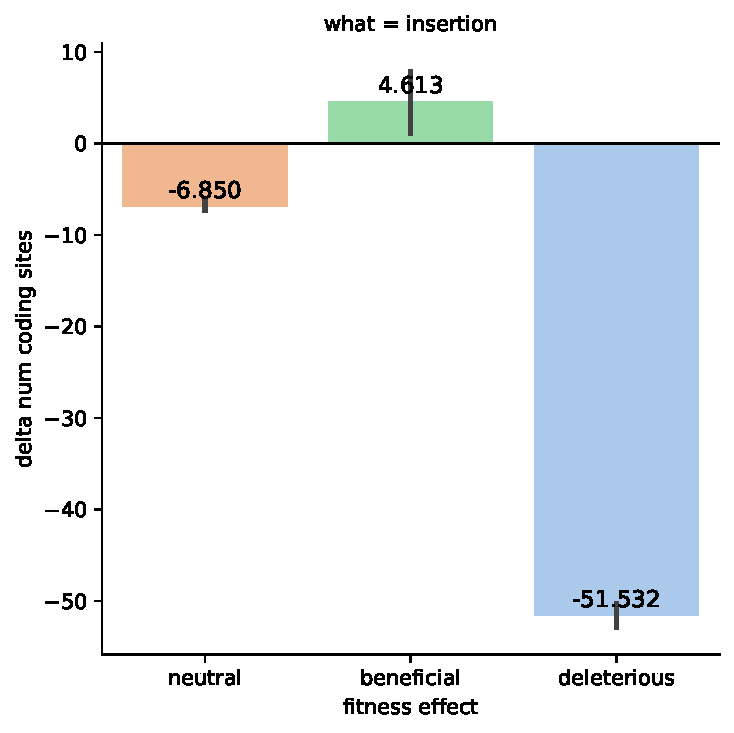
\includegraphics[width=0.5\linewidth]{binder/binder/teeplots/col=what+hue=fitness-effect+kind=bar+palette=pastel+textlabels=True+viz=catplot+x=fitness-effect+y=delta-num-coding-sites+ext=.pdf}%
    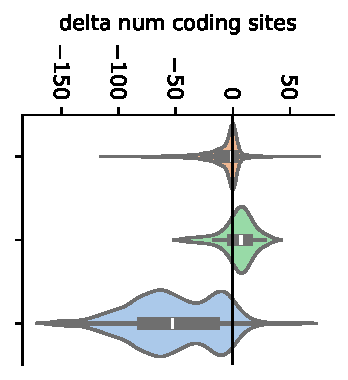
\includegraphics[height=0.5\textwidth, trim={0 0 0 0.6cm}, clip, angle=90]{binder/binder/teeplots/col=what+hue=fitness-effect+kind=violin+palette=pastel+textlabels=True+viz=catplot+x=fitness-effect+y=delta-num-coding-sites+ext=.pdf}
    \caption{\footnotesize change in coding site count by neutral, beneficial, and deleterious slip duplications; violin plots show count delta distributions and bar plots show mean count deltas}
    \end{subfigure}

\begin{minipage}{\linewidth}
    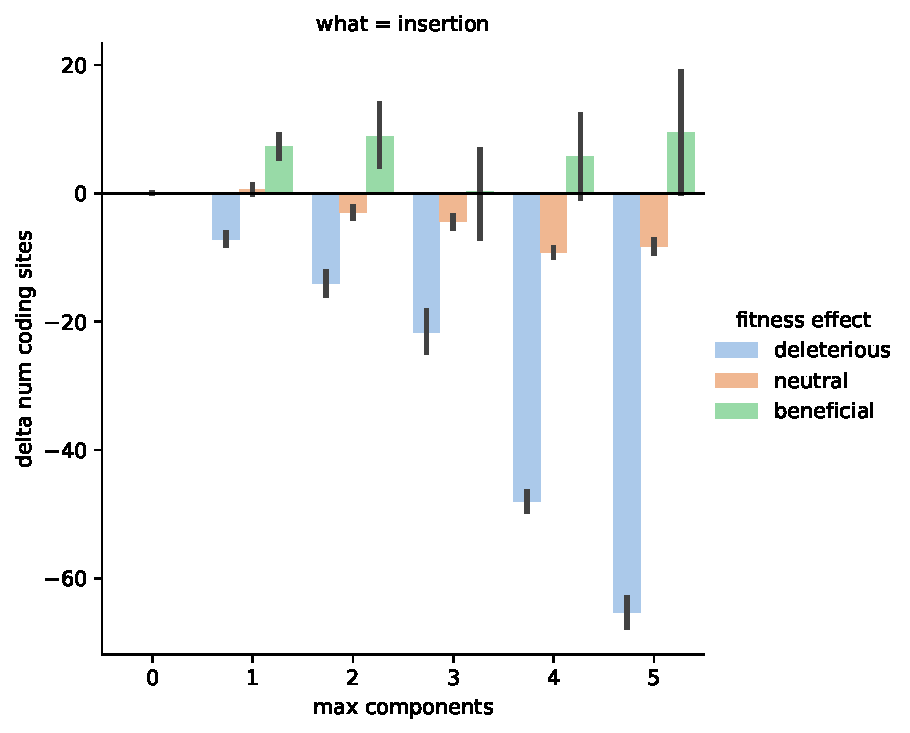
\includegraphics[width=0.35\linewidth, trim={0 0 3.3cm 0}, clip]{binder/binder/teeplots/col=what+hue=fitness-effect+kind=bar+palette=pastel+viz=catplot+x=max-components+y=delta-num-coding-sites+ext=.pdf}
    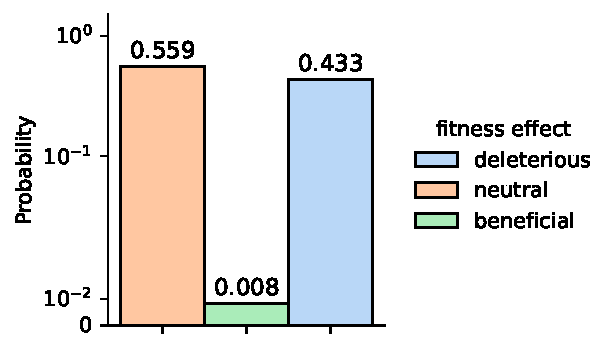
\includegraphics[width=0.64\linewidth, trim={0.6cm 0 0 0}, clip]{binder/binder/teeplots/col=what+hue=fitness-effect+kind=hist+multiple=stack+palette=pastel+stat=probability+viz=displot+x=fitness-effect+ext=.pdf}
\end{minipage}

    \begin{subfigure}{0.35\linewidth}
    \caption{\footnotesize  mean change in coding site count by neutral, beneficial, and deleterious slip duplications, disaggregated by maximum task complexity of derived genome}
    \end{subfigure}
    \begin{subfigure}{0.64\linewidth}
    \centering
    \caption{\footnotesize proportion of sampled slip duplications with neutral, beneficial, and deleterious outcomes}
    \end{subfigure}
~\\
    \caption{
        \textbf{Null distribution of insertion mutation outcomes, sampled over slip-duplication treatment lineage histories.}
        \footnotesize
        Notably, insertion mutations that neither add or lose tasks tend to decrease brittleness, reducing the number of task-critical coding sites --- particularly for genomes that have acquired complex tasks.
        Unsurprisingly, deleterious mutations tend to greatly decrease coding site count and beneficial mutations, which add new tasks, tend to increase them.
        Error bars give bootstrapped 95\% CI.
        Data shown from second-phase experiments.
    }
    \label{fig:nulldist}
\end{figure*}
